\documentclass[a4paper, titlepage]{report}
\usepackage[utf8]{inputenc}
\usepackage{courier} % Required for the courier font
\usepackage[bookmarks]{hyperref}
\usepackage{amsfonts}
\usepackage{graphicx}

%redefine percentage sign to be a little smaller
\let\oldpct\%
\renewcommand{\%}{\scalebox{.9}{\oldpct}}

\begin{document}

\title{Artificial Life Individual Assignment}
\author{
	Sigurt Bladt Dinesen
	\\\texttt{sidi@itu.dk}
}

\maketitle

\tableofcontents
\chapter{Evolutionary Computation}
This chapter details my solution to \texttt{Option 2}, using a genetic algorithm
to solve an instance of the Traveling Salesman Problem (TSP).

The source code is provided \href{https://github.com/Bladtman242/GA-TSP}{here}
\footnote{https://github.com/Bladtman242/GA-TSP }. The code is writen as a
literate haskell program, and can as such be read instead of this chapter of the
report. A compiled pdf of the literate program is included with the source.

There are four main points to define a genetic algorithm. Here are the
definitions I used to this lab:
\begin{description}
\item[Genotype and phenotype]
The genotype is just an ordered list of vertexes (city ids).
The interpretation of the genotype (the phenotype) is a path through the graph
representing our instance of TSP, progressing through the vertices in the
genome, returning the first vertex in the end.

\item[Mutation]
The step that takes one generation of genomes, and creates a
new generation of genomes. In this report, mutation is done by sexual
reproduction between two genomes, by random crossover, producing only one child.

I experimented with random mutation as well, but did
not achieve any better results.

\item[Fitness]
Determines the \textit{evolutionary} value of a genome, for use in
\texttt{selection}. The obvious choice for a (fitness) function here is the
travel-cost of the phenotype. Neither mutation nor the definition of the genome
ensures the \textit{validity} of a genome in this solution, i.e. a genome could
look like $\left[1,1,1,1,1,1,1,1,1,1\right]$, which is not just a \textit{bad}
solution, but not a solution at all. So the fitness function must steer the
selection away from such genomes. To achieve this, another term is included in
the fitness function: An exponential function (for smoothness) of the Jaccard
distance between the genome, and the list of all vertexes
($\left[1,2,3,4,5,6,7,8,9,10\right]$). 
The final fitness function of a genome $g$ is defined as

	$$2^{J(g) \cdot T} + pathlength(g)$$

Where $J$ is one minus the Jaccard distance between $g$ and the set of all
vertices, and $T$ is a large constant term to ensure that non-zero Jaccard
distances are weighed heavier than any path length.

\item[Selection]
The step that takes one generation of genomes, and decides who (or whose children)
gets to be part of the next generation of genomes.
In this project, selection is done by taking the best half of the population, and
letting it, and their children, be the new population.
This does not preserve diversity very well, but seems to produce good results
nonetheless.
\end{description}

This genetic algorithm converges on a solution after ca. 15 generations. After ca. 30, the worst and best solutions in the genome remain the same, and are of similar fitness.

\chapter{Sensors and Actuators}
This chapter details our group work for the second lab.
We went with the arduino option, but didn't get very far within the allotted
time.

\section*{Sensors --- Exercise 1}
\subsection*{A light-dependent resistor}
We got our hands on a light-dependent resistor (LDR). LDRs work as regular
resistors, but their resistance differ with the light level around them. The
more light, the lower the resistance. 

\begin{figure}[htbp]
\centering
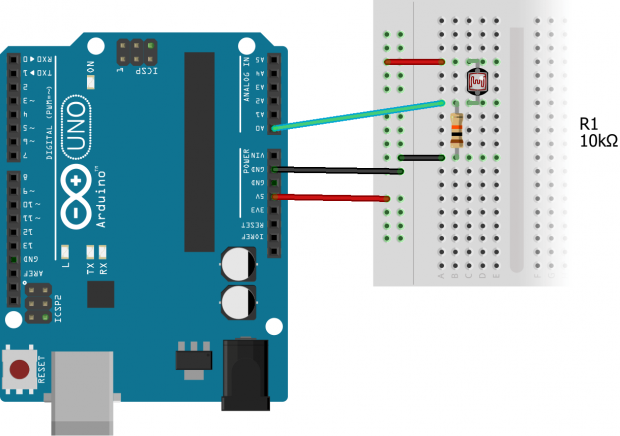
\includegraphics[width=0.8\textwidth]{imgs/Photoresistor/arduino_diagram.png}
\label{fig:photo_circuit}
\caption{}
\end{figure}

\begin{figure}[htbp]
\centering
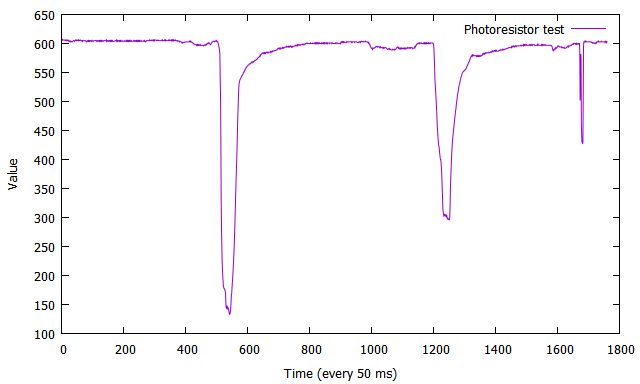
\includegraphics[width=0.8\textwidth]{imgs/Photoresistor/result_photoresistor.png}
\label{fig:photo_plot}
\caption{The, somewhat mistakenly labeled, \textit{Photoresistor test} plot measures voltage over time. Higher voltage means means more light}
\end{figure}

We connected the LDR to the arduino using a voltage divider circuit similar
(though not equivalent) to that in figure \ref{fig:photo_circuit}. Long story
short, the higher the voltage measured, the more light. We logged the values
using the arduino's serial console. The results are plotted in figure
\ref{fig:photo_plot}. The valleys in the plot correspond to (from left to right)
testing with a black object, testing with a white object, and me sitting down
besides the sensor after testing.

As can be seen on the plot, close proximity of dark objects give lower values
than proximity of bright objects. This is due the higher reflectiveness
of bright objects. This can be exploited to distinguish between, say, a black
marker line on white piece of paper, and the rest of that paper (Stay tuned, for
lab 3! (kidding (although that is what lab 3 is about))).

\subsection*{A Potentiometer}
Next we connected a potentiometer to the arduino and, following the
instructions, took measurements at five (or 9, in our case) different positions.

\begin{figure}[htbp]
\centering
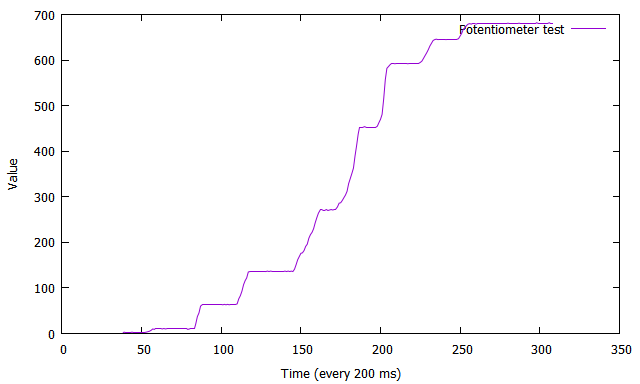
\includegraphics[width=0.8\textwidth]{imgs/Potentiometer/result_pot.png}
\label{fig:pot_plot}
\caption{Measured voltage over the potentiometer, over time.}
\end{figure}

\begin{figure}[htbp]
\centering
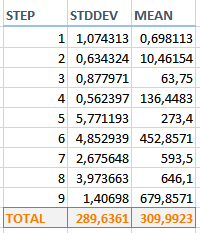
\includegraphics[width=0.4\textwidth]{imgs/Potentiometer/excel_dev.PNG}
\label{fig:fig:stats}
\caption{Measured voltage over the potentiometer, over time.}
\end{figure}

Like LDRs, potentiometers are variable resistors, but their resistance varies
with the position of dial or rod. While the LDR had a lot of noise, the
potentiometer gave stable measurements when left untouched, as seen in figure
\ref{fig:pot_plot}

This story (of stableness) is corroborated by the aggregates over the
measurements shown in figure \ref{fig:stats}, showing low std. deviations.

\section*{A dc motor --- Exercise 2}
Since drivers are for whelps (yes they are yes they are yes they are), we
connected the DC motor using a simple circuit with a zener diode and transistor
to protect the arduino (also; we couldn't find a driver). This still leaves the
DC powered from the arduino though.

After a slow-start period, the motor ran pretty consistently. Braking the shaft
by hand was very easy, indicating that the motor had high RPM but low torque, as
expected. We carefully avoided completely stopping the motor, as doing so will
build up charge/energy internally in the motor, to the point where the heat
buildup melts the insulation of the coils, shorting the motor.

We did not get to try feedback control, as we ran out of time.

\end{document}
